\documentclass[a4paper,11pt]{article}
\usepackage[utf8]{inputenc}
\usepackage[T1]{fontenc}
\usepackage{lmodern}
\usepackage{booktabs}
\usepackage{geometry}
\geometry{margin=1in}
\usepackage{graphicx}
\usepackage{pgfplots}
\pgfplotsset{compat=1.18}
\usepackage{pgfplotstable}
\usepackage{siunitx}
\usepackage{caption}

\title{Calibration Curve — Anemometer}
\author{}
\date{\today}

\begin{document}
\maketitle

\section*{Measurements}
\begin{table}[ht]
\centering
\resizebox{\textwidth}{!}{%
\begin{tabular}{*{7}{S}}
\toprule
\multicolumn{1}{c}{Measurement 1} & \multicolumn{1}{c}{Measurement 2} & \multicolumn{1}{c}{Measurement 3} & \multicolumn{1}{c}{Measurement 4} & \multicolumn{1}{c}{Measurement 5} & \multicolumn{1}{c}{Average Pulses} & \multicolumn{1}{c}{Actual Speed (km/h)}\\
\midrule
7.5 & 6.5 & 6 & 7.5 & 6.5 & 6.8 & 22.74\\
3 & 3.5 & 4 & 3.5 & 3.5 & 3.5 & 17.76\\
1.5 & 1 & 2.5 & 2 & 1.5 & 1.7 & 13.84\\
\bottomrule
\end{tabular}%
}
\caption{Measurements used to build the calibration curve.}
\end{table}

\bigskip

\section*{Plot}
\begin{figure}[ht]
\centering
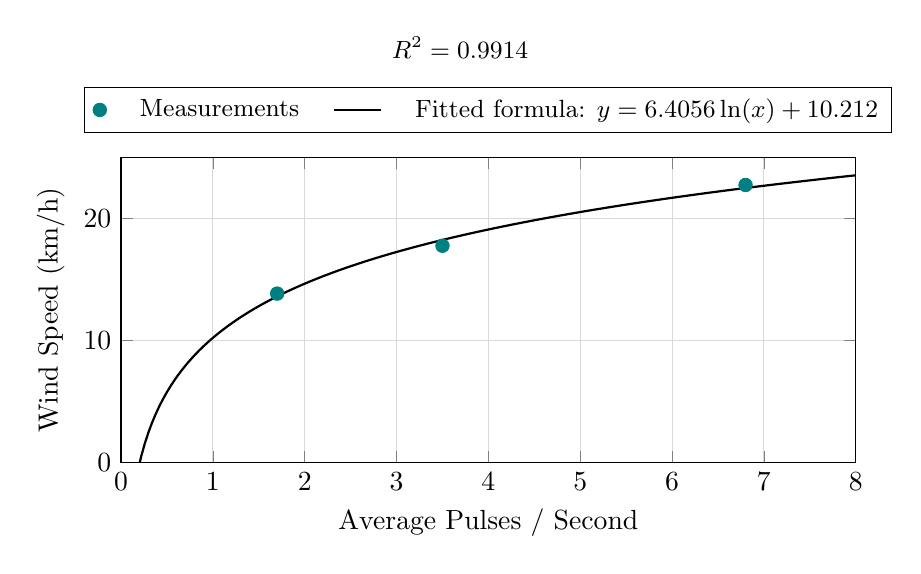
\begin{tikzpicture}
\begin{axis}[
    width=0.9\textwidth,
    height=0.45\textwidth,
    title={Calibration Curve},
    xlabel={Average Pulses / Second},
    ylabel={Wind Speed (km/h)},
    xmin=0, xmax=8,
    ymin=0, ymax=25,
    grid=major,
    grid style={gray!30},
    legend style={
        font=\small,
        cells={align=left},
        at={(0.5,1.08)},
        anchor=south,
        legend columns=-1,
        column sep=1em,
    },
    title style={yshift=1.2ex},
]

% --- Data points (measurements)
\addplot[
    only marks,
    mark=*,
    mark options={scale=1.2},
    color=teal
] table[row sep=crcr] {
x y\\
6.8 22.74\\
3.5 17.76\\
1.7 13.84\\
};
\addlegendentry{Measurements}

% --- Logarithmic fit line (formula)
\addplot[
    domain=0.1:8,
    samples=200,
    color=black,
    thick
] {6.4056*ln(x) + 10.212};
\addlegendentry{Fitted formula: $y=6.4056\ln(x)+10.212$}

\end{axis}

% --- R² label above the plot
\node[font=\small, align=left, yshift=5mm] at (current bounding box.north) {$R^2 = 0.9914$};

\end{tikzpicture}
\caption{Calibration curve: wind speed vs average pulses per second.}
\end{figure}

\end{document}
